\documentclass[20pt,margin=1in,innermargin=-4.5in,blockverticalspace=-0.25in]{tikzposter}
\usepackage[rm]{roboto}
\usepackage[T1]{fontenc}
\geometry{paperwidth=42in,paperheight=30in}
\usepackage[utf8]{inputenc}
\usepackage{amsmath}
\usepackage{isu-theme}
\usepackage{amsfonts}
\usepackage{amssymb}
\usepackage{graphicx}
\usepackage{enumitem}
\usepackage[style=ieee,url=false,doi=false,isbn=false]{biblatex}

\addbibresource{isu-ese.bib}


% set theme parameters
\tikzposterlatexaffectionproofoff
\usetheme{ISUTheme}
\usecolorstyle{ISUStyle}

\title{SIGMA: Systematic Island Grammar forMation Approach\\
Merging Grammars}
\author{Isaac Griffith and Rosetta Roberts}
\institute{Empirical Software Engineering Laboratory\\
College of Science and Technology, Idaho State University}

% begin document
\begin{document}
\maketitle
\centering
\begin{columns}
    \column{0.32}
    \block{Introduction}{
        Motivation---

        Research Goal---

        Research Question---
    }
    \block{Approach}{
        \begin{minipage}[c]{.5\linewidth}
            \begin{center}
                Steps
            \end{center}
            \begin{enumerate}
                \item Parse Grammars
                \item Trivally Merge Grammars
                \item Normalize Grammar \label{normalize_step}
                \item Measure Production Similarities
                \item Merge Most Similar Productions \label{merge_similar_step}
                \item Repeat Steps \ref{normalize_step}--\ref{merge_similar_step} Until Max Similarity is Below a Threshold
                \item Output Grammars
            \end{enumerate}
        \end{minipage}\hfill\begin{minipage}[c]{.5\linewidth}
            \begin{tikzfigure}[Merge Process]
                \label{fig:merge_process}
                \includegraphics[width=\linewidth]{../../papers/merge/images/paper/SIGMA-DFD-vertical.pdf}
            \end{tikzfigure}
        \end{minipage}

        \begin{minipage}[c]{.5\linewidth}
            \begin{center}
                Data Model
            \end{center}
            \begin{itemize}
                \item Object Based
                \item Right Hand Side of Productions is an Object
                \item Constructed via Transformation of Grammar's Abstract Syntax Tree
                \item Converted to Text via Visitor
            \end{itemize}
        \end{minipage}\hfill\begin{minipage}[c]{.5\linewidth}
            \begin{tikzfigure}[Data Model]
                \label{fig:data_model}
                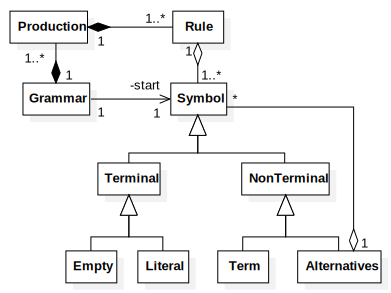
\includegraphics[width=\linewidth]{../../papers/merge/images/paper/diagram.eps}
            \end{tikzfigure}
        \end{minipage}%


        \innerblock{Measuring Production Similarity}{
            \begin{minipage}[t]{.5\linewidth}
                \begin{center}
                    Productions $P_a,P_b$ like \texttt{A`a'B}
                \end{center}
                $$\frac{2|LCS(P_a, P_b)|}{|P_a|+|P_b|}$$

                $LCS$ returns the longest common subsequence.
            \end{minipage}\hfill\begin{minipage}[t]{.5\linewidth}
                \begin{center}
                    Productions $P_a,P_b$ like \texttt{A|`a'|B}
                \end{center}
                $$\frac{2|P_a \cup P_b|}{|P_a|+|P_b|}$$
            \end{minipage}
        }
        
        \innerblock{Normalization}{
            Normalizes grammars so that all rules match one of two forms:

            \texttt{$\texttt{P}_1\rightarrow$ A`a'B}

            \texttt{$\texttt{P}_2\rightarrow$ A|`a'|B}
        }
    }

    \column{0.36}
    \block{Experimental Design}{}
    \block{Results}{
    }
    \column{0.32}
    \block{Discussion}{}
    \block{Conclusions}{}
    
    
    \block{References}{
        \begin{footnotesize}
        \printbibliography[heading=none]
        \end{footnotesize}
    }
    
    \block{Acknowledgements}{
        \begin{footnotesize}
            This research is supported by funding from the Ronald E. McNair Post Baccalaureate Achievement Program at Idaho State University, which is sponsored by the Department of Education (P217A170169).
        \end{footnotesize}
    }
\end{columns}
\end{document}